

\section{Fratture del Collo del Femore}

\subsection{Definizione}

Il \textbf{femore} è il più grande osso lungo del nostro organismo, e
dal punto di vista anatomico può essere generalmente suddiviso in una
\emph{parte centrale}, il \emph{corpo}, detto più propriamente
\textbf{\emph{diafisi}}, e in due estremità, dette
\textbf{\emph{epifisi}}, di cui la prossimale si articola con l'osso
dell'anca formando l'articolazione coxo-femorale, mentre quella distale
si articola con la rotula e la tibia, formando l'articolazione del
ginocchio; le diafisi e le epifisi sono unite tra loro da delle regioni
che prendono il nome di \textbf{\emph{metafisi}}, e che durante
l'adolescenza corrispondono alle aree occupate dalla cartilagine di
accrescimento, che fino alla chiusura delle metafisi consente
l'allungamento dell'osso.
\begin{figure}[!ht]
\centering
	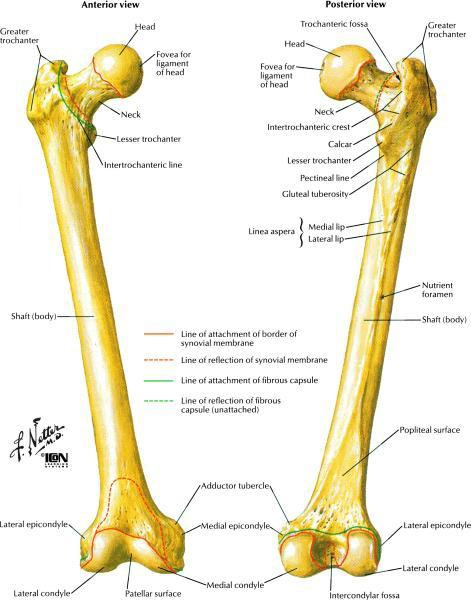
\includegraphics[width=0.5\textwidth]{007/image1.jpeg}
\end{figure}
Quando si parla di \textbf{fratture del collo del femore} si intendono
quindi le fratture che \emph{riguardano l'epifisi prossimale}, la quale
ha una struttura anatomica peculiare e risulta costituita da una
\textbf{testa}, sostenuta da un \textbf{collo}, alla due base di trovano
due prominenze ossee, note come \textbf{grande} \textbf{trocantere} e
\textbf{piccolo} \textbf{trocantere} del femore.

Bisogna inoltre ricordare che per \textbf{\emph{frattura}} si intende
una qualsiasi lesione che causa una \emph{soluzione di continuità
all'interno dell'osso stesso}, determinata da una forza la cui intensità
supera la resistenza elastica dell'osso stesso: in questa definizione
rientrano quindi due variabili principali, che sono appunto
l'\emph{intensità della forza} e la \emph{resistenza dell'osso}, da cui
deriva anche che esistono due forme principali di fratture, le
\textbf{fratture propriamente dette}, in cui la resistenza dell'osso è
normale, ma l'intensità della forza è sufficientemente elevata da
vincerla, e le \textbf{fratture patologiche}, in cui la resistenza ossea
è diminuita, ad esempio a causa di cisti ossee, metastasi tumorali,
osteopetrosi o osteoporosi (in realtà l'osteoporosi non rientra nelle
fratture patologiche propriamente dette, ma è comunque considerata una
condizione borderline), e in tutti questi casi la forza applicata non
avrebbe intensità tale da determinare una frattura in un osso sano, ma
riesce a causarla a causa della marcata compromissione della resistenza
ossea.

Quando poi si parla di \textbf{\emph{osso}}, è importante precisare in
base a quale punto di vista lo si sta valutando, perché per osso si può
intendere o come \emph{organo} (il femore, l'omero, ecc) oppure come
\emph{tessuto}, in questo caso formato da osteoni, componente inorganica
ed organica, deputato a svolgere un'importante funzione meccanica, e
infatti al suo interno la struttura è disposta in \textbf{lamelle
ossee}, le quali non sono collocate a caso, ma sono disposte secondo le
linee di forza che agiscono su quel determinato segmento osseo, e in
particolare a livello del collo del femore abbiamo due fasci principali,
un \emph{fascio principale che contrasta le forze tensive}, teso tra la
testa del femore e la base del grande trocantere, ed un \emph{fascio
principale che contrasta le forze comprensive}, cioè il carico, che va
dalla testa del femore sino alla base del collo, appena sopra al piccolo
trocantere. Questi due fasci si incrociano quindi all'interno del collo,
determinando un'area che in sezione appare triangolare e prende appunto
il nome di \textbf{triangolo di Ward}, ben osservabile nel giovane
adulto, ma che con l'invecchiamento e l'osteoporosi tende ad
ingrandirsi, determinando purtroppo una riduzione della resistenza in
quest'area.
\begin{figure}[!ht]
\centering
	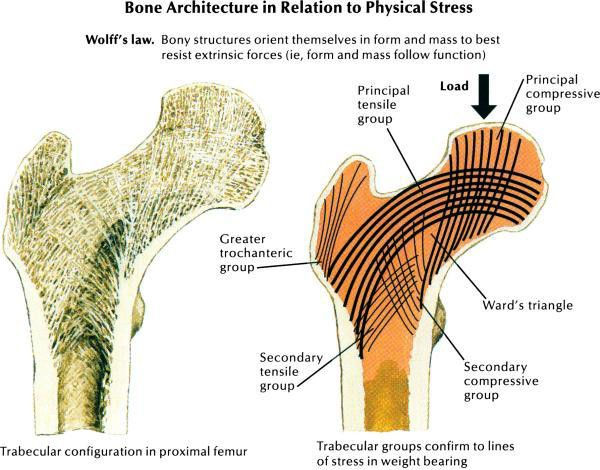
\includegraphics[width=0.5\textwidth]{007/image2.jpeg}
\end{figure}
\subsection{Epidemiologia delle Fratture del Collo del Femore}

Dal punto di vista epidemiologico, si tratta di fratture che sono
piuttosto frequenti nell'\emph{età avanzata}, mentre sono più rare nei
giovani, e purtroppo nell'anziano la frattura del collo del femore è una
condizione che tende ad aggravare le altre patologie concomitanti in
maniera anche molto significativa. Sempre dal punto di vista
epidemiologico, tuttavia, bisogna anche precisare che nei soggetti
giovani, la frattura mediale del collo femorale è tipicamente correlata
con traumi ad alta energia, quali possono essere incidenti
motociclistici, il pattinaggio o gli sci, e sono condizioni altamente
problematiche, poiché le fratture mediali determinano spesso una necrosi
ischemica della testa del femore.

\subsection{Osteoporosi}


Si intende per osteoporosi la riduzione della massa ossea nell'ambito
del nostro apparato scheletrico. Bisogna ricordare però che l'osso è un
organo biologico costituito da cellule, a funzione meccanica, ed è per
questo che possono essere inserite viti al suo interno, perché possiede
una resistenza meccanica. Nel corso della vita, la fisiologia del
tessuto osseo fa sì che questo si modifichi: la parte tubulare dell'osso
si allarga in diametro ma aumenta il canale midollare, determinando una
riduzione della sua resistenza in quanto si avrà uno squilibrio tra
posizione e riassorbimento con prevalenza del riassorbimento osseo (ecco
perché da giovani si hanno mani più piccole: con l'invecchiamento le
falangi si allargano divenendo più deboli dal punto di vista meccanico).
Queste modifiche però, non vanno considerate come patologiche, ma come
fisiologia nell'ambito dell'invecchiamento: questo vale per tutti gli
organi (potrebbe entrare nell'ambito della patologia qualora trovassimo
la cura). L'osteoporosi, quindi, non è considerabile una vera e propria
patologia, anche se ovviamente le considerazioni variano in base al
contesto in cui si colloca, ad esempio è ovvio che l'osteoporosi in una
pz di 50 anno alla quale sono stati tolti utero ed ovaie per fibromi a
25 anno, non può essere considerata fisiologica.

\subsection{Classificazione delle Fratture del Collo del Femore}


Esistono diverse classificazioni delle fratture del collo femorale, ma
la più importante dal punto di vista didattico è quella \emph{su base
anatomica}, che le suddivide, rispetto alla linea intertrocanterica, in:

\begin{itemize}
\item
  \textbf{\emph{Fratture Mediali}}, che sono quelle che avvengono
  medialmente all'inserzione della capsula articolare, verso la linea
  mediana;
\item
  \textbf{\emph{Fratture Laterali}} e \textbf{\emph{Pertrocanteriche}},
  che si hanno al di fuori della capsula e sulla linea
  intertrocanterica.
\end{itemize}

Questa classificazione è importantissima dal punto di vista prognostico,
perché \emph{le fratture mediali possono determinare interruzione della
vascolarizzazione a livello della testa del femore}, in quanto si ha una
lesione a livello capsulare, mentre le pertrocanteriche e le laterali
presentano una prognosi migliore perché non determinano un'interruzione
della vascolarizzazione di questo distretto. La capsula articolare,
infatti, può essere vista come un tubo o una guaina che stabilizza
l'articolazione coxo-femorale e possiede, oltre all'inserzione a livello
del bordo circonferenziale del cotile, anche un'inserzione a livello
della linea intertrocanterica: questa disposizione è molto importante
perché si riflette anche sulla \textbf{vascolarizzazione}, infatti la
vascolarizzazione del collo femorale deriva in gran parte dalle
\emph{arterie circonflesse anteriori} e dall'\emph{arteria circonflessa
posteriore}, mentre la vascolarizzazione della testa è a carico di rami
che si dipartono sempre dall'arteria circonflessa, la quale decorre nel
punto in cui la capsula articolare si inserisce a livello della linea
intertrocanterica, e anche dell'\emph{arteria del legamento rotondo},
che deriva dall'arteria otturatoria, la quale nel 60-70\% dei casi con
la maggiore età va incontro ad obliterazione. Da questa peculiare
vascolarizzazione ne deriva che una frattura che interrompe la
vascolarizzazione a livello della teste determina in genere ischemia con
possibile necrosi, ma se l'individuo con questo tipo di frattura ha la
fortuna di possedere l'arteria del legamento rotondo pervia, la frattura
può anche non andare incontro a necrosi, ecco perché non tutte le
fratture mediali del collo femorale esitano nella necrosi ischemica
della testa del femore.
\begin{figure}[!ht]
\centering
	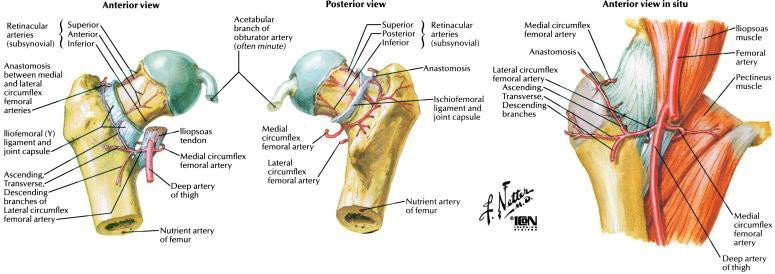
\includegraphics[width=0.8\textwidth]{007/image4.jpeg}
\end{figure}

\subsection{Meccanismo Traumatico delle Fratture del Collo Femorale}


In genere, le cause di questo tipo di fratture sono condizioni
relativamente banali, come \emph{cadute in casa}, o in condizioni o
luoghi pericolosi, ma va tenuto a mente che \textbf{spesso il paziente
cade perché si frattura, e non il contrario}: in seguito ad un
inciampamento, ad esempio, il femore subisce una \emph{torsione}, con
\emph{improvviso aumento del carico che determina la frattura}, che a
sua volta causa un'\emph{impotenza funzionale improvvisa ed il paziente
cade}. È inoltre importante capire se il paziente è caduto perché si è
rotto il femore o se ha avuto un TIA, e per discriminare tra le due
condizioni è bene fare alcune valutazioni, ad esempio se è presente
anche una frattura del polso si deve pensare ad una reazione di difesa,
per cui il paziente era cosciente e ha cercato di attutire la caduta,
mentre se vi è una frattura a livello del viso, la rottura del naso o un
ematoma del volto si deve pensare ad un TIA, perché non c'è stata
probabilmente alcuna risposta di difesa da parte del paziente.

\subsection{Fratture Mediali}


Le fratture mediali del femore possono a loro volta essere sotto
classificate in:

\begin{itemize}
\item
  \textbf{\emph{Fratture Mediali Sottocapitate}}, che interessano la
  porzione più alta del collo femorale, appena sotto alla testa;
\item
  \textbf{\emph{Fratture Mediali Mediocervicali}}, che interessano la
  porzione intermedia del collo;
\item
  \textbf{\emph{Fratture Mediali Basocervicali}}, che sono poste alla
  base del collo, e sono delle fratture borderline, nel senso che non è
  sempre facile discriminarle dalle fratture pertrocanteriche.
\end{itemize}
\begin{figure}[!ht]
\centering
	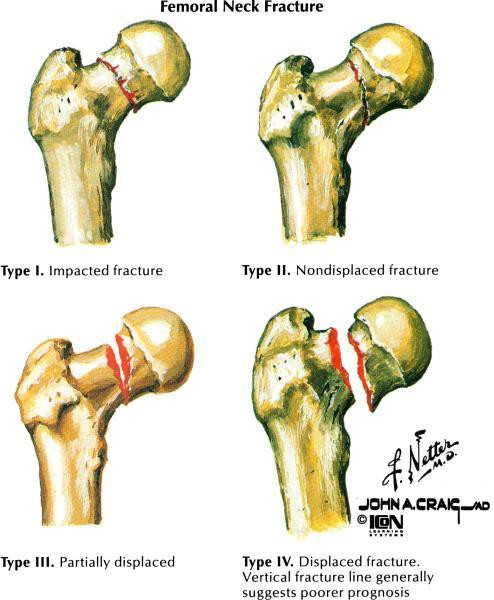
\includegraphics[width=0.5\textwidth]{007/image5.jpeg}
\end{figure}
Esistono anche altre sottoclassificazioni, come la
\textbf{\emph{classificazione di Garden}} {[}vedi Internet{]}, che
distingue le fratture in base al \emph{movimento traumatico},
suddividendole in \textbf{fratture per abduzione}, in cui l'arto
inferiore viene abdotto in modo forzato, e in \textbf{fratture per
adduzione}, in cui il paziente cade con la coscia sotto al bacino e si
ha una adduzione forzata..
\begin{figure}[!ht]
\centering
	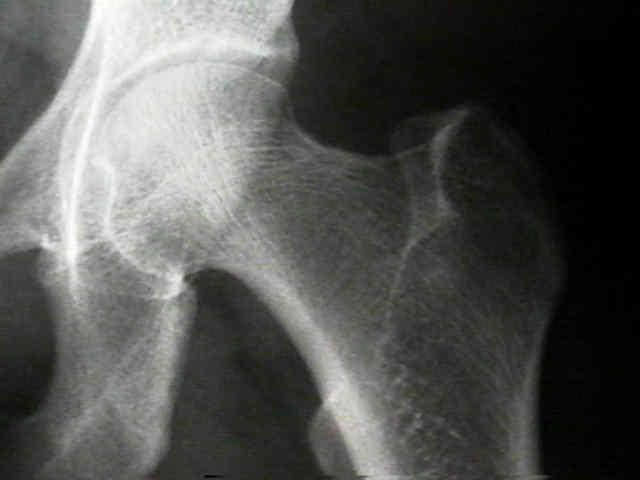
\includegraphics[width=0.5\textwidth]{007/image6.jpeg}
\end{figure}
\paragraph{Quadro Clinico}

Per quanto riguarda il quadro clinico, non esistono differenze molto
significative tra fratture mediali e laterali, sebbene vi possano essere
alcune sfumature sintomatologiche; il \textbf{dolore}, dovuto
all'intensa stimolazione delle fibre nervose del periostio, è molto
intenso e localizzato in \emph{sede inguinale}, ma può avere una
localizzazione più ampia se la frattura è esposta e si ha anche
lacerazione delle parti molli circostanti. Peculiare è poi
l'\textbf{extrarotazione dell'arto}, atteggiamento tipico della fratture
dell'epifisi femorale prossimale, sia mediale che laterale, con
\textbf{accorciamento di tutto l'arto} ed \textbf{impotenza funzionale}
nella flessione dell'anca a ginocchio esteso, in quanto qualsiasi
frattura del collo del femore, non permette la manovra di elevazione di
tutto l'arto senza flettere il ginocchio. Nonostante ciò, è bene tenere
a mente che alcuni pazienti con fratture di tipo Garden I, cioè
ingranate e ben composte, riescono comunque a camminare, sono
relativamente stabili e riferiscono solo un dolore in sede inguinale, e
in questi casi la diagnosi può richiedere una TC, in quanto all'Rx solo
un occhio esperto è in grado di vedere che le lamelle ossee hanno un
orientamento diverso tra loro.
\begin{figure}[!ht]
\centering
	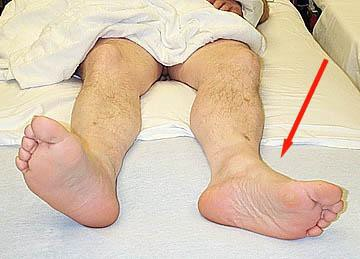
\includegraphics[width=0.5\textwidth]{007/image9.jpeg}
\end{figure}


\paragraph{Quadro Radiografico}

All'Rx, è necessario fare sempre due proiezioni ortogonali, una
\emph{antero-posteriore} e l'altra \emph{latero-laterale}, quest'ultima
in realtà chiamata \textbf{proiezione} \textbf{inguinale}, poiché
effettuata tramite proiezioni ginecologica dell'altro arto. Segni
radiologici valutabili confrontando l'arto patologico con quello
controlaterale sano sono i seguenti:

\begin{itemize}
\item
  In proiezione inguinale si vede bene l'\emph{extrarotazione dell'arto
  col grande trocantere spostato verso il basso};
\item
  Si può osservare un'\emph{interruzione delle lamelle ossee}, che
  permette di valutare anche le fratture composte, le quali hanno
  comunque un rischio non indifferente di andare incontro a
  scomposizione;
\item
  \emph{L'angolo tra collo e diafisi, in genere di 125\textsuperscript{o}, è aumentato},
  soprattutto nel confronto con l'arto controlaterale;
\item
  In proiezione inguinale, \emph{l'asse del collo non viene mantenuto};
\item
  La \textbf{\emph{linea di Shenton}}, cioè la linea che congiunge la
  parte inferiore della branca ileo pubica alla parte mediale del collo
  del femore, \emph{è interrotta per la presenza di una deviazione in
  varo del collo}.
\end{itemize}
\begin{figure}[!ht]
\centering
	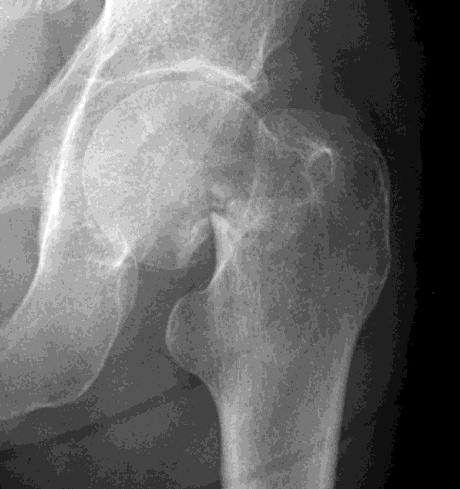
\includegraphics[width=0.5\textwidth]{007/image10.png}
\end{figure}
\subsection{Fratture Laterali del Collo Femorale}


Anche in questo caso, possono essere sotto classificate in diversi tipi:

\begin{itemize}
\item
  \textbf{\emph{Fratture Laterali Basicervicali}}, cioè fratture
  borderline che si possono riscontrare anche nelle mediali;
\item
  \textbf{\emph{Fratture Laterali Transtrocanteriche}};
\item
  \textbf{\emph{Fratture Laterali Pertrocanteriche}}, che sono le
  comuni, tanto da essere considerate le fratture laterali per
  antonomasia. A volte possono essere fratture comminute, in cui si
  stacca solo il piccolo trocantere perché tirato dal muscolo ileopsoas.
\item
  \textbf{\emph{Fratture Laterali Isolate dei Trocanteri}}, che non sono
  fratture articolari e sono tipiche dei ciclisti; nei casi più
  complessi si può osservare la testa del femore che sfonda la lamina
  quadrilatera del bacino, creando delle lesioni gravissime
\item
  \textbf{\emph{Fratture Laterali Sottotrocanteriche}}.
\end{itemize}

Dal punto di vista clinico la sintomatologia è sovrapponibile a quella
riscontrata nelle fratture mediali, con dolore in sede inguinale,
impotenza funzionale nella flessione dell'arto a ginocchio esteso,
accorciamento dell'arto, extrarotazione. Tipica è poi la presenza di
\emph{ecchimosi} e di \emph{ematomi}: le ecchimosi si presentano come
soffusioni emorragiche a livello di cute e sottocute, mentre gli ematomi
sono raccolte di sangue in una cavità non preformata (altrimenti sarebbe
un emartro o un'altra condizione specifica), ma all'interno di un
muscolo o del sottocute, e dal punto di vista semiologico l'ematoma è
facile da riconoscere perché si presenta come un ``bozzo'' apprezzabile
alla palpazione, che si muove rispetto ai tessuti limitrofi. Se una
frattura mediale non è molto scomposta e non rompe la capsula, il sangue
che esce dall'osso fratturato rimane dentro la capsula e non si creano
né ecchimosi né ematoma; se invece la frattura è pertrocanterica, cioè
posta al di fuori della capsula, lo stravaso ematico che segue la
frattura può andare a colonizzare il sottocute, determinando la
formazione appunto di ecchimosi ed ematomi.

\subsection{Terapia e Complicanze delle Fratture del Collo Femorale}


Il trattamento delle fratture del collo del femore è ovviamente
condizionato dalle eventuali comorbilità del paziente, ad esempio in un
diabetico in trattamento adeguato con poche unità di insulina o con
ipoglicemizzanti orali, a seguito della frattura si può avere uno
scompenso metabolico che mette fuori controllo il diabete, poiché si
sviluppa una sindrome da adattamento con attivazione dell'asse
ipotalamo, ipofisi-surrene ed con un aumento dei livelli circolanti di
cortisolo, che causa appunto insulino-resistenza e fa sì che il diabete
non sia più ben controllabile, oppure in caso di un paziente
cardiopatico, uno stimolo intensamente doloroso come la frattura può
determinare lo sviluppo di uno scompenso cardiaco, per cui bisogna
sempre tenere conto del contesto in cui si va ad agire.

Dopo la diagnosi, quindi, la prima cosa che si dovrebbe fare è la
\textbf{trazione a zampale}, cioè una trazione modesta, di non più di 2
Kg, per cercare di dominare l'atteggiamento extra-rotatorio determinato
dalla frattura del collo del femore, in particolare dalla rottura del
segmento intertrocanterico, e quindi cercare di ridurre il dolore, così
da dominare anche la contrattura muscolare e l'accorciamento.

Il trattamento delle fratture del collo femorale, inoltre, è un
\emph{approccio prettamente chirugico}, che in molti ospedali viene
eseguito in urgenza (entro 3 giorni) o al più in urgenza differita
(entro 7 giorni). In generale, proprio a causa delle comorbilità, prima
si opera, meglio i pazienti stanno (a Parma si cerca di operare entro le
prime 12-24 ore se possibile, così da evitare la sindrome da
allettamento o lo sviluppo di piaghe da decubito, infezioni delle vie
urinarie e TEP). Lo scopo del trattamento è quindi quello di
\emph{ridurre il più possibile il periodo di allettamento},
\emph{consentire una mobilizzazione precoce} e \emph{ridurre di
conseguenza le complicanze generali} (N.B.: La frattura del collo del
femore, in soggetti anziani, è una condizione molto grave, che provoca
complicanze potenzialmente letali, per cui, anche se l'intervento non è
scevro da rischio, è comunque bene tentarlo per dare al paziente un
chance di sopravvivere). È ovvio però che prima di procedere
all'intervento il paziente deve essere stabilizzato, in particolare
bisogna cercare di correggere il più possibile la glicemia e le
ipopotassiemie, così da rendere l'intervento il meno rischioso
possibile.

L'intervento chirurgico avviene in due passaggi:

\begin{enumerate}
\def\labelenumi{\arabic{enumi}.}
\item
  \textbf{Riduzione della Frattura}, in cui si rimettono a posto i
  frammenti , affrontando il problema dell'extrarotazione, per cui si
  devono esercitare delle forze uguali e contrarie a quelle della
  scomposizione, vale a dire trazione ed intrarotazione;
\item
  \textbf{Osteosintesi/Fissazione}, che può essere interna con placche,
  viti o chiodi, oppure esterna, che consiste nella fissazione senza
  ferite chirurgiche, applicando delle fiches transcutanee nel collo del
  femore, a livello della diafisi, il tutto collegato ad un fissatore
  esterno (in genere si preferisce ricorrere alla fissazione esterna
  quando la ferita è esposta, cioè quando non è possibile agire
  stabilizzandola internamente.
\end{enumerate}

\subsubsection{Trattamento delle Fratture Mediali}


Per le fratture mediali esistono \emph{3 opzioni di trattamento} a
seconda del tipo di lesione e della capacità funzionale del paziente:
\begin{figure}[!ht]
\centering
	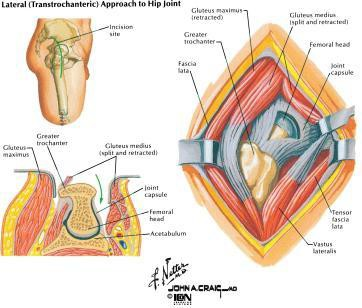
\includegraphics[width=0.5\textwidth]{007/image13.jpeg}
\end{figure}
\begin{figure}[!ht]
\centering
	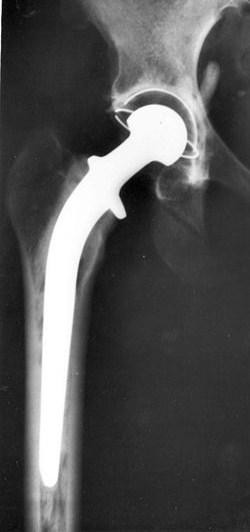
\includegraphics[width=0.2\textwidth]{007/image15.jpeg}
\end{figure}
\begin{itemize}
\item
  Per le \textbf{fratture mediali meno scomposte}, quindi con
  \emph{minor rischio di necrosi}, si conserva la testa e si fissa la
  frattura mediante osteosintesi con viti e placche, e questa procedura
  viene in genere effettuata tramite applicazione di due viti di
  titanio, parallele su di un piano e divergenti sull'altro, così da
  evitare la rotazione (in genere bastano due viti, perché si deve
  cercare di ridurre al minimo il rapporto tra osso e quantità di
  metallo, così da non svuotare la testa). In alternativa, per le
  \textbf{fratture basicervicali}, vengono usate viti e placche, con una
  vite più grossa ed una più piccola per evitare la rotazione. In questo
  caso la sintesi viene effettuata se il malato possiede capacità
  funzionale elevata ed ha la possibilità di stare un paio di mesi con
  le stampelle, per poi effettuare una protesi in un secondo momento se
  non migliora.
\item
  In caso di \textbf{frattura mediale in paziente con una capacità
  funzionale discreta} si applica un'\emph{endoprotesi}, cioè si
  sostituisce la testa, mettendola in rapporto col cotile originario. Si
  tratta quindi di una protesi parziale, ed è un intervento tipico di
  chi possiede appunto una capacità funzionale discreta ma non
  eccezionale, perché alla lunga si può sviluppare una
  \emph{cotiloidite}, cioè l'osso a livello del cotile si usura e fa
  male.
\item
  In caso di \textbf{frattura molto scomposta e ad elevato rischio di
  necrosi} \textbf{in una persona ad elevata capacità funzionale} si fa
  un'\emph{artroprotesi}, che consiste nella sostituzione della testa e
  del cotile, con lo stesso procedimento seguito per la coxatrosi: prima
  si incide la cute ed il sottocute, arrivando alla fascia lata che
  viene incisa, poi si scollano i muscoli glutei dal grande trocantere e
  si evidenzia, con l'uso di leve apposite, la capsula articolare in
  extrarotazione, la quale viene incisa a croce e tagliata attorno al
  cotile. A questo punto la testa del femore viene lussata e rimossa con
  appositi strumenti; il collo viene tagliato via con un seghetto e
  rifinito con seghe pneumatiche, poi si elimina il cotile originario
  tramite delle frese circolari e lo si sostituisce col cotile
  protesico, mentre a livello dello stelo femorale viene inserita
  l'endoprotesi. Infine, in caso di endoprotesi si mette la testa e si
  fa la riduzione senza componente acetabolare, mentre in caso di
  endoprotesi totale si fa la manovra al contrario. L'intervento si
  conclude con la sutura dei muscoli, della fascia lata e della cute.
\end{itemize}

\subsubsection{Trattamento delle Fratture Laterali}


Le fratture laterali hanno un braccio di leva molto diverso rispetto a
quelle mediali e di solito il trattamento viene effettuato tramite
\emph{viti e placche}, di cui esistono diversi modelli; il trattamento
chirurgico in questo caso prevede un'incisione più spostata verso il
ginocchio, più bassa rispetto al trocantere, e le placche vengono poi
inserite con angoli di inclinazione diversi a seconda della
conformazione dell'anca, mettendo un filo guida con trapani ad alta
velocità e si fa l'alloggio per il vettore grande, e lo si inserisce.
Tutti questi passaggi sono effettuati sotto al controllo di un
amplificatore di brillanza, uno strumento che presenta una visione
invertita rispetto alla radiologia tradizionale (cioè l'osso appare nero
invece che bianco), e nelle fratture pertrocanteriche è importante
mettere la vite nel quadrante inferiore, così da evitare che essa esca
dalla testa come conseguenza di un processo osteoporotico.
\begin{figure}[!ht]
\centering
	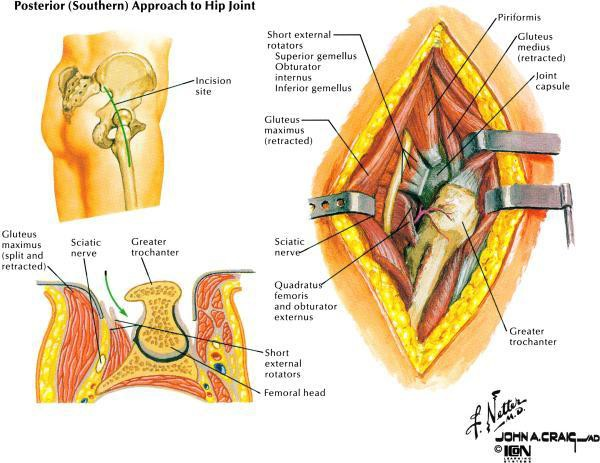
\includegraphics[width=0.5\textwidth]{007/image16.jpeg}
\end{figure}
\subsubsection{Trattamento Post-Operatorio}

Dopo il trattamento chirurgico, si deve procedere ad una
\emph{rieducazione funzionale non appena la ferita guarisce}, anche se
in realtà, se la comorbilità è bassa ed il montaggio buono, il paziente
con endoprotesi o con un chiodo gamma può essere messo un piedi subito.
La rieducazione funzionale è solo una parte della fisioterapia, e si
intende con questa definizione anche la rieducazione alla funzione della
deambulazione. È tuttavia ovvio che pazienti con fratture che non danno
garanzie di stabilità devono rimanere allettati per un certo periodo di
tempo, ma \emph{la fisioterapia è una componente importantissima che
deve essere iniziata il prima possibile}.

\subsubsection{Complicanze delle Fratture del Collo del Femore}

Le complicanze delle fratture del collo femorale, così come nelle
fratture generali, possono essere generalmente suddivise in
\textbf{complicanze generali} e \textbf{complicanze locali}:

\begin{itemize}
\item
  \textbf{\emph{Complicanze Generali}}: Si caratterizzano per un
  \emph{decadimento delle condizioni generali}, soprattutto in ambito
  geriatrico, perché il paziente diventa completamente dipendente dagli
  altri, ed anche l'aspetto psicologico grava significativamente sul
  paziente, con possibile insorgenza di depressione senile e conseguente
  scarsa motivazione alla fisioterapia.
\item
  \textbf{\emph{Complicanze Locali}}: Sono più frequenti nelle fratture
  mediali, e sono rappresentate essenzialmente dalla \emph{necrosi
  ischemica della testa del femore}, tipicamente in presenza di fratture
  molto scomposte, in cui è l'arteria del legamento rotondo è
  obliterata. Spesso si tenta comunque una sintesi, ma la necrosi può
  comparire dopo l'intervento, in un lasso di tempo che arriva anche a
  12 mesi, per cui è un'eventualità che va sempre tenuta in
  considerazione. Altra complicanza locale tipica delle fratture mediali
  è lo sviluppo di una \emph{pseudoartrosi}, condizione in cui alla
  testa del femore arriva una quantità ridotta di sangue, abbastanza per
  non dare necrosi, ma non sufficiente a garantirne la guarigione.
\end{itemize}

